%Copyright 2014 Jean-Philippe Eisenbarth
%This program is free software: you can 
%redistribute it and/or modify it under the terms of the GNU General Public 
%License as published by the Free Software Foundation, either version 3 of the 
%License, or (at your option) any later version.
%This program is distributed in the hope that it will be useful,but WITHOUT ANY 
%WARRANTY; without even the implied warranty of MERCHANTABILITY or FITNESS FOR A 
%PARTICULAR PURPOSE. See the GNU General Public License for more details.
%You should have received a copy of the GNU General Public License along with 
%this program.  If not, see <http://www.gnu.org/licenses/>.

%Based on the code of Yiannis Lazarides
%http://tex.stackexchange.com/questions/42602/software-requirements-specification-with-latex
%http://tex.stackexchange.com/users/963/yiannis-lazarides
%Also based on the template of Karl E. Wiegers
%http://www.se.rit.edu/~emad/teaching/slides/srs_template_sep14.pdf
%http://karlwiegers.com
\documentclass{scrreprt}
\usepackage{listings}
\usepackage{underscore}
\usepackage[bookmarks=true]{hyperref}
\usepackage[utf8]{inputenc}
\usepackage[english]{babel}
\usepackage{amsmath}
\usepackage{amssymb}
\usepackage{tikz}
\usetikzlibrary{calc,patterns,angles,quotes}
\hypersetup{
    bookmarks=false,    % show bookmarks bar?
    pdftitle={Software Requirement Specification},    % title
    pdfauthor={Raphael Pfaff},                     % author
    pdfsubject={TeX and LaTeX},                        % subject of the document
    pdfkeywords={TeX, LaTeX, graphics, images}, % list of keywords
    colorlinks=true,       % false: boxed links; true: colored links
    linkcolor=blue,       % color of internal links
    citecolor=black,       % color of links to bibliography
    filecolor=black,        % color of file links
    urlcolor=purple,        % color of external links
    linktoc=page            % only page is linked
}%
\def\myversion{1.0 }
\date{}
%\title
\usepackage{hyperref}
\begin{document}

\begin{flushright}
    \rule{16cm}{5pt}\vskip1cm
    \begin{bfseries}
        \Huge{REQUIREMENTS\\ SPECIFICATION}\\
        \vspace{1.9cm}
        for\\
        \vspace{1.9cm}
        FH Aachen Park Railroad Loco\\
        \vspace{1.9cm}
        \LARGE{Version \myversion approved}\\
        \vspace{1.9cm}
        Prepared by Raphael Pfaff\\
        \vspace{1.9cm}
        FH Aachen\\
        \vspace{1.9cm}
        \today\\
    \end{bfseries}
\end{flushright}

\tableofcontents


\chapter*{Revision History}

\begin{center}
    \begin{tabular}{|c|c|p{10cm}|c|}
        \hline
	    Name & Date & Reason For Changes & Version\\
        \hline
	    Pfaff & 03.04.2020 & Emission of new document & 1.0\\
        \hline
	    Pfaff & \today & Added strength requirements, component weight, concept documentation requirements &  1.1 \\
        \hline
    \end{tabular}
\end{center}

\chapter{Introduction}

\section{Purpose}
This document describes the requirements for the FH Aachen rail vehicle engineering lab locomotives.
\section{Document Conventions}
\textbf{Bold face is used for critical features or dimensions}

\section{Intended Audience and Reading Suggestions}
This document is intended for FH Aachen's suppliers at all levels.

\section{Project Scope}
The product is intended to operate in the FH Aachen rail vehicle lab, mainly to test autonomous driving functionalities. A potential use in the IMechE railway challenge is optional.

\section{References}
- IMechE railway challenge specification 2019 edition

\chapter{Overall Description}
\section{Product Perspective}
The product shall operate in the lab continuously as well as in open environments.

\section{Product Functions}
The locomotive shall be able to propel trains without local emissions. It shall be able to operate on tracks with small track radii.

The locomotive shall provide interfaces for LiDAR scanners and cameras. 

The locomotive shall have automatic couplers on both ends.

\section{User Classes and Characteristics}
Users will be students and staff of FH Aachen.

\section{Operating Environment}
Inside environment:
\begin{itemize}
	\item Temperature: $15\ldots30^\circ\mathrm{C}$
	\item Humidity: $0\ldots100^\circ\mathrm{\%}$
\end{itemize}

Outside environment as per IMechE specifications.

\section{Design and Implementation Constraints}
The locomotive shall be handleable with 1 person, except for carrying.

The locomotive shall have an attractive outward appearance.

\section{User Documentation}
Proof of car body strength and safety against derailment shall be provided with the vehicle. Full design files shall be accessible.
 
\section{Assumptions and Dependencies}
A standard drive train and brake control equipment can be assumed:
\begin{itemize}
		\item 48 V power supply
		\item Electrical motors Dunker BG95x40, up to 4
		\item Pneumatic brake supply, de-energise to a activate
		\end{itemize}

\chapter{External Interface Requirements}
\section{User Interfaces}
The following status shall visible to the user:
\begin{itemize}
	\item Brake applied/released
	\item Wheel blocked
\end{itemize}

\section{Hardware Interfaces}
Coupler system interface are 4 M8 bolts as depicted in Figure \ref{fig:coupler}:
\begin{figure}[htbp]
\begin{center}
\begin{tikzpicture}
 \draw[rounded corners = 5mm] (0,0) -- (12,0) -- (12,8) -- (0,8) -- cycle;
\draw (2,2) circle (.45);
\draw (10,2) circle (.45);
\draw (2,6) circle (.45);
\draw (10,6) circle (.45);
\draw[<->] (0,1) -- (12,1) node[pos = 0.5, above] {120};
\draw[<->] (1,0) -- (1,8) node[pos = 0.5, above, rotate = 90] {80};
\draw[<->] (2,2) -- (10,2) node[pos = 0.5, above] {80};
\draw[<->] (2,2) -- (2,6) node[pos = 0.5, above, rotate = 90] {40};
\end{tikzpicture}
\caption{Coupler system interface}
\label{fig:coupler}
\end{center}
\end{figure}

It shall be possible to fit an external sensor system by help of 4 M8 bolts in a $\Box \,100$ pattern to both vehicle fronts and the the top.

The car body shall provide space for the following installations:
\begin{itemize}
		\item Battery system according to specification
		\begin{itemize}
		\item Size of battery module: W190 x D361 x H125 mm
		\item 2 (optionally 4) Modules to be placed in vehicle
		\item Weight per module 15 kg
		\end{itemize}
		\item Control system (app. (300x300x200)mm$^3$), weight < 20 kg
		\item Compressor D\"urr D30 with reservoir (10 l)
\end{itemize}

\section{Software Interfaces}
n/a

\section{Communications Interfaces}
n/a


\chapter{System Features}
Only additional features are listed in the sequel.
\section{F1: Reduced curve radius}

\subsection{Description and Priority}
For operation in the lab and on the test track, reduced curve radii must be negotiated by the vehicle.

\subsection{Stimulus/Response Sequences}
n/a

\subsection{Functional Requirements}


REQ-1: For operation in the lab, a 5 m curve radius must be negotiated.

REQ-2: For operation on the test track, a 10 m radius must be negotiated at a minimum velocity of 10 km/h.
\newpage
\section{F2: Visibility for LiDAR system}
\subsection{Description and Priority}
It is desirable to provide 360$^\circ$ vision to the Ouster OS1-32 LiDAR sensor without obstruction in the space envelope described in the IMechE specification.

\subsection{Stimulus/Response Sequences}
n/a

\subsection{Functional Requirements}
REQ-3: The field of view for a top mounted LiDAR system shall remain free from obstructions, while maintaining the gauge from IMechE. Field of view is depicted in Figure \ref{fig:lidar} with $\theta = 16.6^\circ$.
\begin{figure}[htbp]
\begin{center}
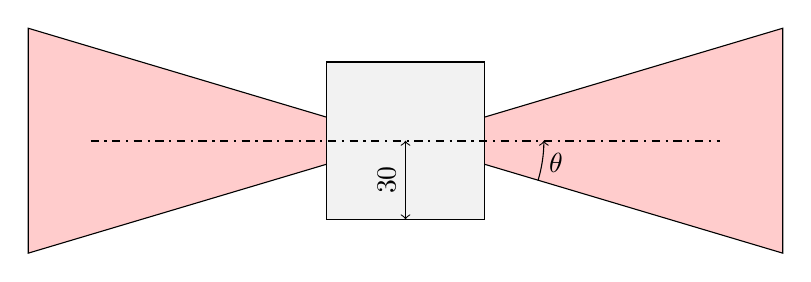
\begin{tikzpicture}
 \coordinate (o) at (0,0);
  \draw[fill = red!20]  (0,0) -- (-16.6:5) coordinate (b) -- (16.6:5)- - cycle;
   \draw[fill = red!20] (0,0) -- (-16.6:-5) -- (16.6:-5)- - cycle;
   \draw[fill = gray!10] (-1,-1) -- (1,-1) -- (1,1) -- (-1,1) -- cycle;
\draw[thick, dashdotted]  (-4,0) -- (4,0) coordinate(a);
\pic [draw, ->, "$\theta$", angle eccentricity=1.1, angle radius = 50] {angle = b--o--a};
\draw[<->] (0,-1) -- (0,0) node[pos = 0.5, above, rotate = 90] {30};
\end{tikzpicture}
\caption{LiDAR field of view}
\label{fig:lidar}
\end{center}
\end{figure}



\chapter{Nonfunctional Requirements}
\section{Strength requirements}
The vehicle shall be designed according to static strength requirements as per EN12663-1 for locomotives. For strength requirements given by a force, a scaling factor of $s_{F} = \frac{1}{5^3}$ shall be applied. Proof of strength shall be provided for the following cases:
\begin{itemize}
		\item Buff and draft forces (Section 6.2.2 of EN 12663-1)
		\item Vertical load (Section 6.3.1 of EN 12663-1)
		\item Lifting (Section 6.3.2 of EN 12663-1)
		\end{itemize}

\section{Concept documentation}
The concept documentation provided for the IDR milestone shall provide the following information:
\begin{itemize}
	\item Description of the concept including specific features
	\item Outward appearance and dimensions:
	\begin{itemize}
		\item Length, width and height
		\item Estimated mass
		\item Wheel base
		\item Pivot distance
	\end{itemize}
	\item Installation spaces
	\begin{itemize}
		\item Dimensions
		\item Accessibility
		\end{itemize}
	\item Cost estimate
	\item Open issues in the specification
	\item Risks in the development process and mitigation measures
\end{itemize}


Documentation shall be provided as presentation (\LaTeX or PowerPoint).
\section{Performance Requirements}
n/a

\section{Safety Requirements}
n/a
\section{Security Requirements}
n/a

\section{Software Quality Attributes}
n/a

\section{Business Rules}
n/a

%\chapter{Other Requirements}
%n/a
\end{document}
